\clearpage
\newpage
\noindent\\
\thispagestyle{empty}
\begin{center}
\Large
\begin{flushright}
\vspace{17cm} {\Huge \em{ \textbf{\textcolor{ultramarine}{TALLERES}}}} \\ [0.5cm]
\addcontentsline{toc}{section}{Talleres}
\end{flushright}
\normalsize
\end{center}

\small
\clearpage
\pagestyle{fancy}
\SetHeader{Talleres}{\textit{Congreso Interamericano de Estadística}}

%--------------------------------------------------------------------------
\renewcommand{\titulo}{¿SON REALMENTE CENSOS LOS CENSOS POR REGISTROS?}
\renewcommand{\presentador}{DR. ALPHONSE L. MACDONALD}
\addcontentsline{toc}{subsubsection}{\titulo. \presentador}
\vspace*{1cm}

\begin{center}
\textbf{\textcolor{ultramarine}{\titulo \\}}
\bigskip
\textit{\presentador \\}
\bigskip
\end{center}

\noindent Este taller propone revisar, en grupos de trabajo, las definiciones y características del censo tradicional y del censo por registro, con el objetivo de determinar si el censo por registros puede ser considerado como censo. A través del estudio de diversos documentos, partiendo desde recomendaciones del Congreso Internacional de Estadística de 1853 hasta los recientes manuales de Naciones Unidas, se comparan definiciones, se determinan criterios para la igualdad de conceptos y se arriba a una conclusión.

\begin{table}[H]
\centering
\begin{tabular}{m{0.25\textwidth}  m{0.7\textwidth}}
\begin{center} 
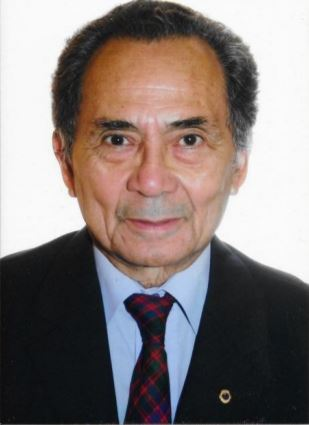
\includegraphics[width=0.2\textwidth]{./fotos/alphonse} \end{center} & 
\noindent \small{Alphonse L. MacDonald, ciudadano de Suriname, Doctor de la Universidad Radboud, Nimega, Países bajos. Especialista en metodología de la investigación, censos, encuestas de hogares y en la planificación económica. Participó en dos proyectos de estadísticas internacionalesinventores: la Encuesta Mundial de Fecundidad (WFS) y el Programa para Desarrollar la Capacidad Nacional de Efectuar Encuestas por Hogares (NHSCP). Ocupó altos cargos técnicos y de representación en las Naciones Unidas en África, América y Europa. Se retiró de la ONU en 2004, pero sigue activo como consultor independiente. Además sigue siendo Consejero Principal (metodología) de la Oficina General de Estadística (ABS) de Suriname.} \\
\end{tabular}
\end{table}

%--------------------------------------------------------------------------
\newpage
\clearpage
\renewcommand{\titulo}{APRENDIENDO DISTRIBUCIONES DE MUESTREO MEDIANTE SIMULACIÓN}
\renewcommand{\presentador}{MG. GUILLERMO SABINO}
\addcontentsline{toc}{subsubsection}{\titulo. \presentador}
\vspace*{1cm}

\begin{center}
\textbf{\textcolor{ultramarine}{\titulo \\}}
\bigskip
\textit{\presentador \\}
\bigskip
\end{center}

\noindent Las distribuciones en el muestreo es un tema muy teórico y abstracto vinculado a la inferencia estadística. Esta abstracción implica que su enseñanza requiera de bastante tiempo y dedicación, ya que es una temática de difícil comprensión. Las nuevas tecnologías informáticas permiten acercar este concepto a los estudiantes didácticamente. La simulación de muestras aleatorias provenientes de una distribución
normal permite comprender el origen y uso de las distribuciones T-student, ChiCuadrado y F-Snedecor de manera amigable. De esta forma se pretende que el estudiante incorpore intuitivamente conceptos tales como grados de libertad, independencia entre media y desvío, intervalos de confianza, sesgo, consecuencias del incremento del tamaño muestral – entre otras – mediante gráficos y medidas de resumen ya estudiadas en estadística descriptiva.

\begin{table}[H]
\centering
\begin{tabular}{m{0.25\textwidth}  m{0.7\textwidth}}
\begin{center} 
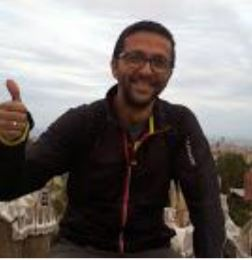
\includegraphics[width=0.2\textwidth]{./fotos/sabino} \end{center} & 
\noindent \small{Guillermo Sabino es Profesor Adjunto de la Universidad Nacional del Comahue, Profesor en Matemáticas y Mg. en Estadística Aplicada egresado de dicha universidad. Comparte con el resto de sus compañeros docentes la inquietud acerca de la forma en la que los estudiantes adquieren los conocimientos, tarea que ha llevado al grupo de trabajo a utilizar diferentes estrategias y materiales didácticos en búsqueda de resultados favorables. Actualmente es Director del Departamento de Estadística de la UNCo y Secretario del Grupo Argentino de Biometría, donde divulga y aprende nuevos conocimientos.} \\
\end{tabular}
\end{table}

%--------------------------------------------------------------------------
\newpage
\clearpage
\renewcommand{\titulo}{VARIACIONES AZAROSAS EN EL AULA DE ESTADÍSTICA}
\renewcommand{\presentador}{DRA. LILIANA TAUBER Y ESP. SILVANA SANTELLÁN}
\addcontentsline{toc}{subsubsection}{\titulo. \presentador}
\vspace*{1cm}

\begin{center}
\textbf{\textcolor{ultramarine}{\titulo \\}}
\bigskip
\textit{\presentador \\}
\bigskip
\end{center}

\noindent Desde algunos años, la comunidad de educadores estadísticos ha expresado su preocupación por lograr una Alfabetización Estadística para todos, enfatizando el desarrollo de propuestas de enseñanza basadas en las ideas fundamentales de la Educación Estadística: aleatoriedad, variabilidad y distribución. Es por ello, que en esta oportunidad, presentaremos una actividad que permite desarrollar estas ideas a través de distintos niveles educativos, utilizando simulaciones con material manipulable y virtual. Además, aportaremos un análisis conceptual de dicha actividad de tal manera de poder reflexionar sobre los conceptos, sus propiedades y relaciones que se pueden introducir a través de la misma.

\begin{table}[H]
\centering
\begin{tabular}{m{0.25\textwidth}  m{0.7\textwidth}}
\begin{center} 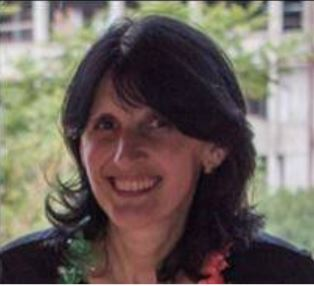
\includegraphics[width=0.2\textwidth]{./fotos/tauber} \end{center} & 
\noindent \small{Liliana Tauber, es Profesora en Matemática, egresada de la Universidad Nacional del Litoral y Doctora en Didáctica de la Matemática por la Universidad de Sevilla. El tema de su Tesis doctoral ha sido: “La Construcción del Significado de la Distribución Normal a partir de actividades de análisis de datos”. Se ha desempeñado como Profesora Titular de Estadística y Métodos Cuali-Cuantitativos en la Carrera de Licenciatura en Psicología de la Universidad Católica de Santa Fe. Desde 1994, se ha desempeñado como profesora de Estadística para diversas carreras, en la Facultad de Humanidades y Ciencias de la Universidad Nacional del Litoral, en la cual actualmente es Profesora Titular. Se especializa en la investigación sobre Educación Estadística, área en la cual ha sido directora de diversos proyectos de investigación desde 2003.} \\
\begin{center} 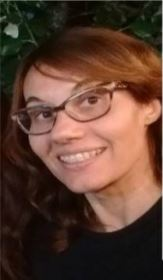
\includegraphics[width=0.2\textwidth]{./fotos/santellan} \end{center} & 
\noindent \small{Silvana Santellán es Profesora de Matemática, egresada en la Universidad Nacional del Litoral y Especialista Docente en Educación Superior y TIC. Actualmente se encuentra desarrollando su tesis para la Maestría en Didáctica Específica de la Facultad de Humanidades y Ciencias, UNL. Desde el año 2008 se ha desempeñado como profesora de cátedras de Estadística en carreras universitarias. ActualmenteesDocente Adjunta en
la cátedra Métodos de Investigación Cuali- Cuantitativos en la carrera de Licenciatura en Psicología de la Universidad Católica de Santa Fe y Ayudante de Cátedra en “Métodos Estadísticos para las Ciencias Sociales”
de Licenciatura en Sociología y en “Estadística I” de la Licenciatura en Biodiversidad, ambas de la Universidad Nacional del Litoral. Además, desde el año 2014 se ha involucrado en la formación de futuros profesores de Matemática y de Nivel Primario. Desde el año 2006 ha participado en distintos proyectos de investigación sobre Educación Estadística.} \\
\end{tabular}
\end{table}

% anterior, en una pagina con items
%\vspace*{1cm}
%\centerline{\textbf{\LARGE{\textcolor{ultramarine}{Talleres}}}}
%\vspace{1cm}

%\begin{itemize}
%\item \textbf{Aprendiendo distribuciones de muestreo mediante simulación} \\
%Mg. Guillermo Sabino \\
%Orientado a docentes de nivel terciario/universitario

%\item \textbf{Variaciones azarosas en el aula de Estadística} \\
%Dra. Liliana Tauber y Esp. Silvana Santellán \\
%Orientado a docentes de nivel secundario

%\item \textbf{¿Son realmente censos los censos por registros?} \\
%Dr. Alphonse L. MacDonald \\
%Orientado a estudiantes.
%\end{itemize}